\documentclass{article}
\usepackage{graphics}
\usepackage{hyperref}
\usepackage{clrscode}
\usepackage{colortbl}
\usepackage{fullpage}
\usepackage{times}
\bibliographystyle{plain}

\pdfinfo{
  /Author (Casey Marshall)
  /Title  (Efficient and safe data backup with Arrow)
  /CreationDate (D:20080606212000)
  /Subject (Data Backup)
  /Keywords (content-addressable storage;error-correcting storage systems;data backup;deduplication)
}

\begin{document}
\title{Efficient and safe data backup with Arrow}
\author{Casey Marshall \\
  University of California, Santa Cruz \\
%\footnote{This work was done in
%    fulfilment of the project requirements for the Master's degree in
%    Computer Science.} \\
%  \texttt{casey.s.marshall@gmail.com}}
  \texttt{csm@soe.ucsc.edu}}

\maketitle

\begin{abstract}
  We describe Arrow, an efficient, safe data backup system for
  computer networks. Arrow employs techniques of delta compression (or
  deduplication) to achieve efficient storage and bandwidth
  utilization, and collision-resistant hashing and error-correction
  coding to protect against and correct storage errors.

  \medskip

  \noindent\textbf{keywords:} content-addressable storage;
  error-correcting storage systems; data backup; deduplication.
\end{abstract}

\section{Introduction}

Content-addressable storage, error detection and correction, and
deduplication are all interesting topics in the field of archival data
storage. Particularly in the case where files are being archived over
time, where snapshots of the file tree are taken, and where there is
significant data in common between snapshots.

Arrow implements a data backup system that combines
collision-resistant hash functions, rolling checksums, and
error-correction codes to provide a deduplicating, versioned,
error-recoverable archival storage system. Arrow stores files as lists
of checksums, and performs a fast checksum search algorithm for
determining what parts of a file have changed, achieving both a
speedup in time to store a version, and a savings in the amount of
physical storage used. There checksums are also used to identify and
verify the integrity of data stored in the system, and
error-correction codes are present to allow correction of small
storage errors.

\section{Related Work}

Rsync is a popular free software program for synchronizing similar
files on computers connected on a network, using a novel checksum
search algorithm to reduce the amount of data that needs to be
transmitted~\cite{tridge:thesis, tridge:96}. Arrow borrows heavily
from rsync, using a similar algorithm to search for duplicate chunks
in files to be backed up, and uses the same rolling checksum
function. The delta-compression ideas behind rsync have inspired other
data backup solutions, implemented simply as thin layers on the rsync
program itself~\cite{rsnapshot}, or as new implementations of the
idea~\cite{rdiff-backup}.

Error-correction codes have been widely used in digital storage and
transmission, prominently in media like compact disks and DVDs, since
the media is exposed to more physical abuse. The sharp increases in
hard drive density and speed, and the relative stability of hard disk
failure rates, have meant that errors in disk storage systems have
become much more frequent. Hard disks also offer error-correction
codes for the data stored to disk, but these error codes are not
portable, are vendor-specific, and are often un-verifiable by
high-level software. A very common error-correction code is the
Reed-Solomon code, which is used today in many digital storage
platforms. With the increasing rates in hard disk failure, focus has
shifted towards fault-tolerant and repair-driven systems, e.g. chunkfs
\cite{henson06chunkfs}.

File snapshotting and content-addressable storage appear in many
systems for file versioning, storage and network optimization,
intelligent caching, and so on, and the design of Arrow follows these
systems.  Elephant~\cite{elephant-sosp} replaces single file inodes
with a log of inodes to keep each change to files, and so it keeps all
versions of files through modifications. Venti~\cite{quinlan02venti}
references parts of files primarily by a strong hash code of short
blocks of data, avoiding duplication of data written to disk.
Ivy~\cite{ivy:osdi02} uses logs of changes and hash code references to
blocks to implement an efficient peer-to-peer network file system.
The Shark file system \cite{shark:ndsi05} optimizes network file
transfer with hashes of data chunks, and intelligent file chunking.
The Git distributed revision control system uses a mutable index and a
write-only object store to implement revision control
\cite{git08wiegley}.

\section{Overview}

Arrow stores files in three separate layers, each managing some part
of the source file tree. The \emph{file tree} layer mirrors the source
file tree, with a same-named directory per source directory, and a
symbolic link per source file. The target of the symbolic link is a
\emph{version file,} which describes a list of chunks that comprise
the file, and contains a reference to the previous version of the
file. The \emph{chunks} are stored in an object storage system where
the key is derived from the chunk's hash code. The overall goal of
Arrow is to use chunk hashes to reduce the amount of data stored and
transferred over the network, and to strongly protect stored data from
corruption by providing enough information to detect and correct
errors.

Figure~\ref{figure:arrow-layout} illustrates the overall layout of
Arrow; the following sections explain how each layer is implemented.

\begin{figure}[ht!]
  \begin{center}
    \scalebox{.5}{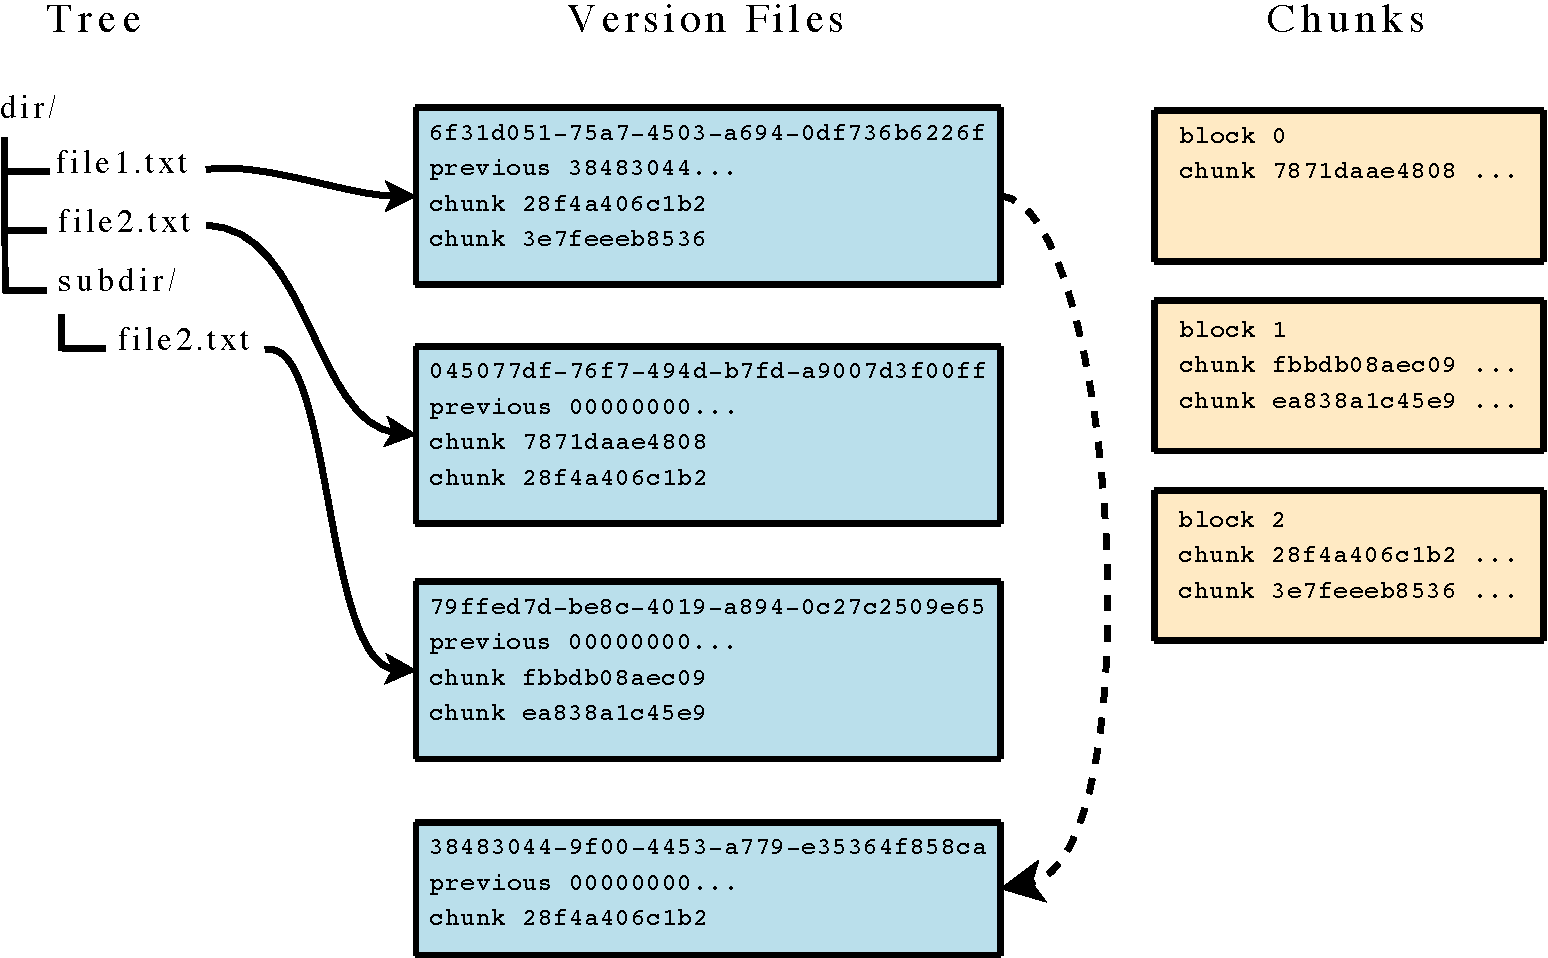
\includegraphics{arrow-layout.pdf}}
    \caption{Overview of how Arrow stores files}
    \label{figure:arrow-layout}
  \end{center}
\end{figure}

\section{Chunk Storage}

Arrow stores files as \emph{chunks,} which are small runs of data from
files (between 700 and 16000 bytes), and chunks are identified by a
pair of hash codes over the data. The hash pair consists of a four
byte simple checksum, similar to Adler-32, which has a \emph{rolling}
property: given a checksum over values \( [m,n] \), it is simple to
compute the sum over values \( [m+1,n+1] \), if we have bytes \( m \)
and \( n+1 \). The other hash is the 16-byte MD5 hash of the data. The
concatenation of these two values is the chunk identifier.

To store chunks, Arrow uses a simple file format shown in
figure~\ref{fig:store-layout}. The store begins with a simple header;
followed by a fixed number of block keys, along with the offset and
length of each chunk, and the size of the key space is chosen once at
store creation time; then the chunk values; the file ends with parity
bytes computed over the rest of the file, using a Reed-Solomon error
correction code.

\begin{figure}[ht!]
  \begin{center}
    \scalebox{.6}{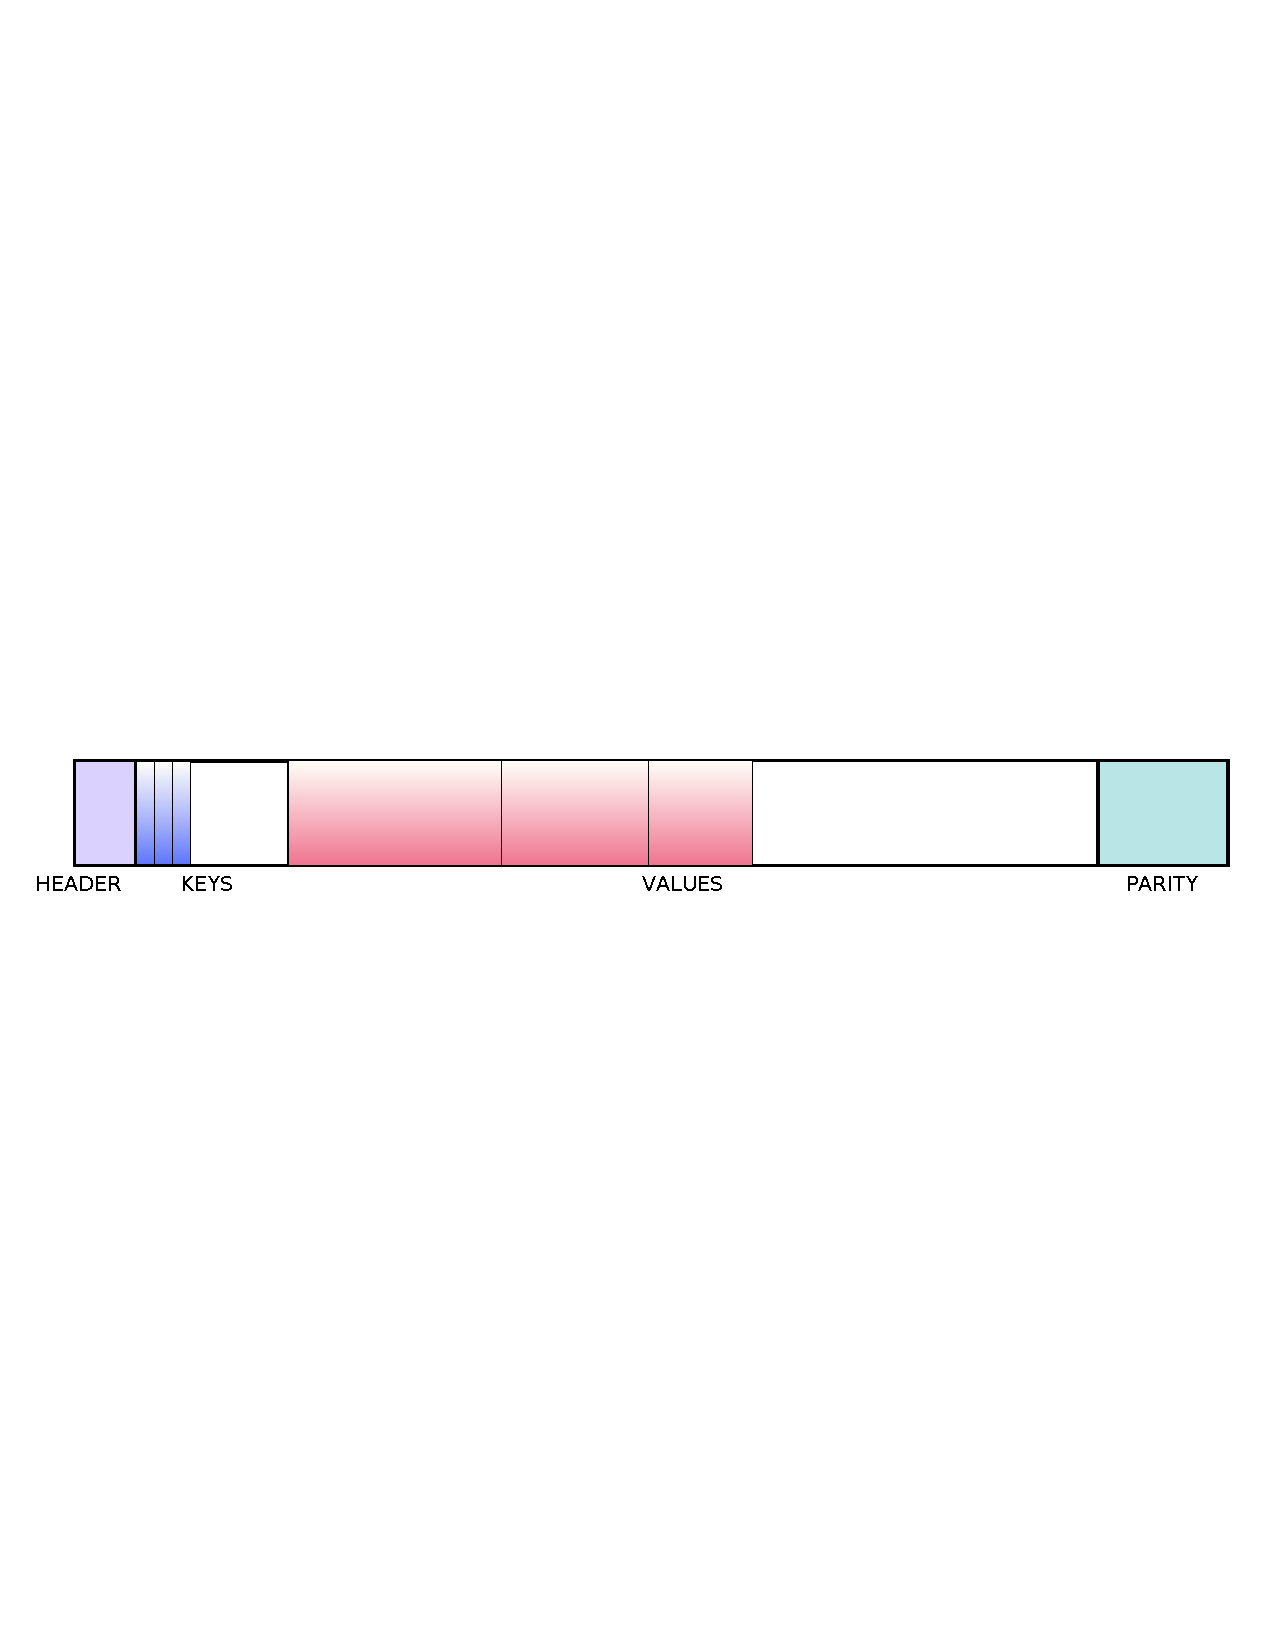
\includegraphics{store-layout.pdf}}
    \caption{Storage layout in arrow.}
    \label{fig:store-layout}
  \end{center}
\end{figure}

Each of these chunk files --- called \emph{blocks} --- is relatively
small; large enough to store up to about 200 chunks, assuming that
chunks average between 700 and 16000 bytes. The key space in a block
is fixed-size; if needed, the data space will grow if it isn't of
sufficient size. We would quickly fill up a single block, so we need
to store chunks across multiple blocks and have a method for managing
them. The technique used by Arrow is \emph{linear hashing,} first
proposed by Witold Litwin in \cite{litwin80}. Core to linear hashing
is the function that maps chunk keys to block identifiers, given in
figure~\ref{proc:linear-hash}.

\begin{figure}[ht!]
\begin{codebox}
\Procname{\proc{linear-hash}(K)}
\li \( x\gets K \bmod 2^i \)
\li \If \( x < n \)
\li  \Then
\li   \( x \gets K \bmod 2^{i+1} \)
    \End
\li \Return \( x \)
\end{codebox}
\caption{The linear hash function}
\label{proc:linear-hash}
\end{figure}

\( i \) and \( n \) are initially zero. If we fill up a block beyond a
``load factor'' --- in Arrow, if 70\% of the slots in the block are
filled --- we add a new block \( n + 2^i \), rehash each key in block
\( n \), which will move some keys from block \( n \) to block \( n +
2^i \), and increment \( n \). Once \(n = 2^i\), we increment \( i \)
and set \( n\gets 0 \). The keys are effectively random, given the
nature of MD5, so rehashing the keys of a block should move
approximately half the entries into the new block.

This implementation allows the chunk storage to grow one block at a
time, while maintaining an \(O(1)\) lookup time, and achieves \(O(1)\)
insertions, with an increased cost at regular intervals when a block
needs splitting. the rationale for this being that looking up a chunk
involves a single execution of \proc{linear-hash}, followed by a
linear search through a list of at most 200 chunk keys. This intuitive
analysis does not consider the costs of doing the lookup considering
the underlying file system, however, which can add significant cost to
the operation.

We have a fairly rough strategy for splitting blocks, too: block \( n
\) is the one that gets split, even if some other block overflowed its
load factor. In practice this shouldn't be a problem, since block \( n
\) is necessarily the one that was split least recently, and since our
keys have a uniformly random distribution, block \( n \) will be the
one expected to have the highest load.

Since arrow stores the chunk's hash along with the chunk, storage
errors can be detected easily by iterating through each chunk key,
recomputing the hash on the chunk, and comparing the values. If there
is a mismatch, we know that there is a storage error either in the key
or in the chunk, so we can attepmt to repair storage errors in either
location, using the parity information. Arrow computes \( (253,255) \)
Reed-Solomon codes over 253-byte subblocks, producing 2 parity bytes,
and on an error it will attempt to correct the error in the key or in
the value, by repeatedly attempting to fix the subblocks that overlap
the apparently-corrupt key or value, confirming the fix by checking
the hashes again. Arrow assumes few errors; it can detect large
errors, but won't be able to correct errors spanning more than a few
bytes.

\section{File Storage}

Files in arrow are stored primarily as lists of chunk references, that
is, the hash pair of the chunk, and will store very small runs of data
directly. The layout of a file is as follows:

\begin{itemize}
\item The name of the underlying file.
\item The MD5 hash of the entire file.
\item The identifier of the previous version of this file, if any.
\item The file size, file mode bitset, and modification, status
  change, and creation times.
\item The chunk size used to chunkify the file. This is inherited from
  previous file versions.
\item A list of chunks. Each chunk is either a reference to a chunk
  stored in the chunk storage layer, or (if the chunk is smaller than
  a chunk identifier) the chunk bytes stored directly.
\end{itemize}

Files are identified by a random 16-byte UUID, and files that have no
previous versions are stored with the null UUID (sixteen zero bytes)
as the previous-version UUID. Each of these files is stored as simple
data files in a flat namespace, with the file's UUID as its file name.

File hierarchies are stored to match the underlying file hierarchy,
where directories are stored as-is, with the same name, and files are
stored as symbolic links to the head revision of the file.

This scheme was chosen for its simplicity; there are possible
refinements we could make to storing file and version hierarchies,
such as storing versioned directories as well as files. For example,
when a directory is backed up, not only are files that changed in that
directory committed as new versions, but also the directory as a whole
--- which may include new, modified, or deleted files --- is committed
as a new version of the directory after all changed files are
committed. A scheme like this would better reflect the needs of a
system that stored historical versions, since files in the same
directory are often related, and rolling back to previous versions for
groups of files may make more sense than rolling back single
files. This file tree scheme also ignores deleted files at the moment,
and cannot handle replacing a file with a directory of the same name
(or vice-versa), but none of these are fundamental issues --- they are
just left unimplemented here.

\section{File Synchronization}

When Arrow has a new version of a file to be backed up, it first
fetches the version file of the previous version of the file, which
will be the \emph{basis} file. Each checksum pair \( (\id{weak},
\id{strong} ) \) that is the underlying chunk size long --- through
the backup process, chunks shorter than the base chunk size may be
stored, but these are ignored in the synchronization, which only uses
the underlying chunk size --- is inserted into a hash table with
\(2^{14}\) entries, by taking the weak sum modulo the table size. A
running rolling checksum is taken over the new file version, one byte
at a time, and each time the hash table is probed for that weak
value. If a possible weak checksum is found, an MD5 is computed over
the current chunk, and if \emph{that} matches, we have found a
duplicate chunk reference, and can emit that reference in the new
file.

The pseudocode, with some details omitted, for this process is given
in figure~\ref{code:sync}. The procedures \proc{rollsum-compute} and
\proc{rollsum-rotate} are the rolling checksum algorithm from
\texttt{librsync}~\cite{librsync}. \proc{hash-probe} searches the
hashtable for the weak hash only, and \proc{hash-contains} tells if
the hashtable contains the weak and strong hash combination.


\begin{figure}[ht!]
\begin{codebox}
\Procname{\proc{file-sync}(\id{basis},\id{newfile},\id{input})}
\li \( H \gets \) hashtable of \( 2^{14} \) entries
\li \For each \id{chunk} in \id{basis}
\li \Do\If \( \id{chunk.length} = \id{basis.chunk\_size} \)
\li   \Then \proc{hash-insert}(\id{chunk.id})
      \End
    \End
\li \( \id{buffer} \gets \id{basis.chunk\_size} \) bytes from \id{input}
\li \( \id{weak} \gets \proc{rollsum-compute}(\id{buffer}) \)
\li \While \( \neg \proc{end-of-file}(input) \)
\li \Do\If \( \proc{hash-probe}(H, \id{weak}) \)
\li  \Then \( \id{strong} \gets \proc{MD5}(\id{buffer}) \)
\li    \If \( \proc{hash-contains}(H, (\id{weak}, \id{strong} ) ) \)
\li    \Then insert chunks between the last match and the
\li          current match into \id{newfile}
\li      insert \( (\id{weak},\id{strong}) \) into \id{newfile}
\li      \( \id{buffer} \gets \id{basis.chunk\_size} \) bytes from \id{input}
\li      \( \id{weak} \gets \proc{rollsum-compute}(\id{buffer}) \)
\li      \textbf{continue}
       \End
     \End
\li  \( c \gets \proc{read}(\id{input}) \)
\li  \( \proc{rollsum-rotate}(\id{weak}, \id{buffer}[0], c) \)
\li  add \( c \) to \id{buffer}
\li  remove the first element from \id{buffer}
    \End
\end{codebox}
\caption{File synchronization procedure}
\label{code:sync}
\end{figure}

The consequence of this procedure is that any chunks in both
\id{basis} and the new file to be backed-up will be stored only
once. If any chunks that exist in the new file that were found in
previous versions of any file, then again, that chunk will only be
stored once --- though, it is very unlikely that we will find
duplicate chunks by chance, unless they have specific signatures, such
as a chunk that consists of all zero bytes.

This synchronization procedure is based on the rsync algorithm, though
it presents some limitations to the delta compression that this
version can achieve. Since the rsync algorithm uses a single block
size, and since these block boundaries are fixed in a single file,
there are limits to the number of duplicate blocks between the basis
file and the new file we can find.

\section{Performance Evaluation}

This first test used a simple C program that will synchronize single
files, and that program was used in a Python program to manage the
version files. This test used the Linux kernel
source~\cite{linux:kernel}, starting with version 2.6.23, and applying
each of the 17 patches released for this
kernel. Table~\ref{table:kernel} shows the results of backing up each
patched kernel tree with Arrow. Figures~\ref{graph:per-patch-deltas}
and \ref{graph:time-files} plot the patch size versus Arrow's increase
in backup size, and the time the backup took versus the number of
files that changed in that patch release.

\begin{table}[ht!]
  \begin{center}
    \begin{tabular}{!{\color[rgb]{.5,.5,.5}\vline}r!{\color[rgb]{.5,.5,.5}\vline}r!{\color[rgb]{.5,.5,.5}\vline}r!{\color[rgb]{.5,.5,.5}\vline}r!{\color[rgb]{.5,.5,.5}\vline}r!{\color[rgb]{.5,.5,.5}\vline}r!{\color[rgb]{.5,.5,.5}\vline}} \hline
      \multicolumn{1}{|>{\columncolor[rgb]{.9,.9,.9}}c|}{\textbf{Patch}} &
      \multicolumn{1}{>{\columncolor[rgb]{.9,.9,.9}}c|}{\textbf{Patch Size}} &
      \multicolumn{1}{>{\columncolor[rgb]{.9,.9,.9}}c|}{\textbf{Source}} &
      \multicolumn{1}{>{\columncolor[rgb]{.9,.9,.9}}c|}{\textbf{Backup}} &
      \multicolumn{1}{>{\columncolor[rgb]{.9,.9,.9}}c|}{\textbf{Time}} &
      \multicolumn{1}{>{\columncolor[rgb]{.9,.9,.9}}c|}{\textbf{Files}} \\ \hline
      \rowcolor{white}
       0 &       0 & 252,065,213 & 283,107,750 & 451.08 & 22,530 \\
      \rowcolor[rgb]{.94,.96,.98}
       1 &   3,218 & 252,065,491 & 283,119,871 &  91.83 & 2 \\
      \rowcolor{white}
       2 &  34,402 & 252,066,473 & 283,208,456 &  89.34 & 18 \\
      \rowcolor[rgb]{.94,.96,.98}
       3 &  65,218 & 252,072,178 & 283,362,188 & 102.47 & 53 \\
      \rowcolor{white}
       4 &  94,870 & 252,073,453 & 283,591,942 & 143.06 & 70 \\
      \rowcolor[rgb]{.94,.96,.98}
       5 & 127,389 & 252,077,945 & 283,912,484 & 181.44 & 81 \\
      \rowcolor{white}
       6 & 182,957 & 252,082,973 & 284,389,157 & 193.47 & 115 \\
      \rowcolor[rgb]{.94,.96,.98}
       7 & 187,496 & 252,084,315 & 284,831,665 & 220.82 & 113 \\
      \rowcolor{white}
       8 & 188,895 & 252,084,342 & 285,277,506 & 229.20 & 107 \\
      \rowcolor[rgb]{.94,.96,.98}
       9 & 221,604 & 252,087,238 & 285,811,410 & 238.36 & 132 \\
      \rowcolor{white}
      10 & 284,301 & 252,091,147 & 286,524,145 & 240.94 & 181 \\
      \rowcolor[rgb]{.94,.96,.98}
      11 & 283,078 & 252,091,071 & 287,204,874 & 254.57 & 175 \\
      \rowcolor{white}
      12 & 281,040 & 252,090,640 & 287,865,620 & 256.07 & 158 \\
      \rowcolor[rgb]{.94,.96,.98}
      13 & 283,099 & 252,090,838 & 288,510,953 & 255.74 & 254 \\
      \rowcolor{white}
      14 & 283,830 & 252,090,842 & 289,146,161 & 257.06 & 146 \\
      \rowcolor[rgb]{.94,.96,.98}
      15 & 541,078 & 252,147,239 & 290,212,238 & 265.04 & 228 \\
      \rowcolor{white}
      16 & 541,304 & 252,147,258 & 291,108,027 & 267.25 & 217 \\
      \rowcolor[rgb]{.94,.96,.98}
      \arrayrulecolor[rgb]{.5,.5,.5}
      17 & 555,389 & 252,150,368 & 292,006,750 & 277.29 & 218 \\ \hline
    \end{tabular}
    \caption{Backup test of Linux kernel versions}
    \label{table:kernel}
  \end{center}
\end{table}

\begin{figure}[ht!]
  \begin{center}
    \scalebox{.6}{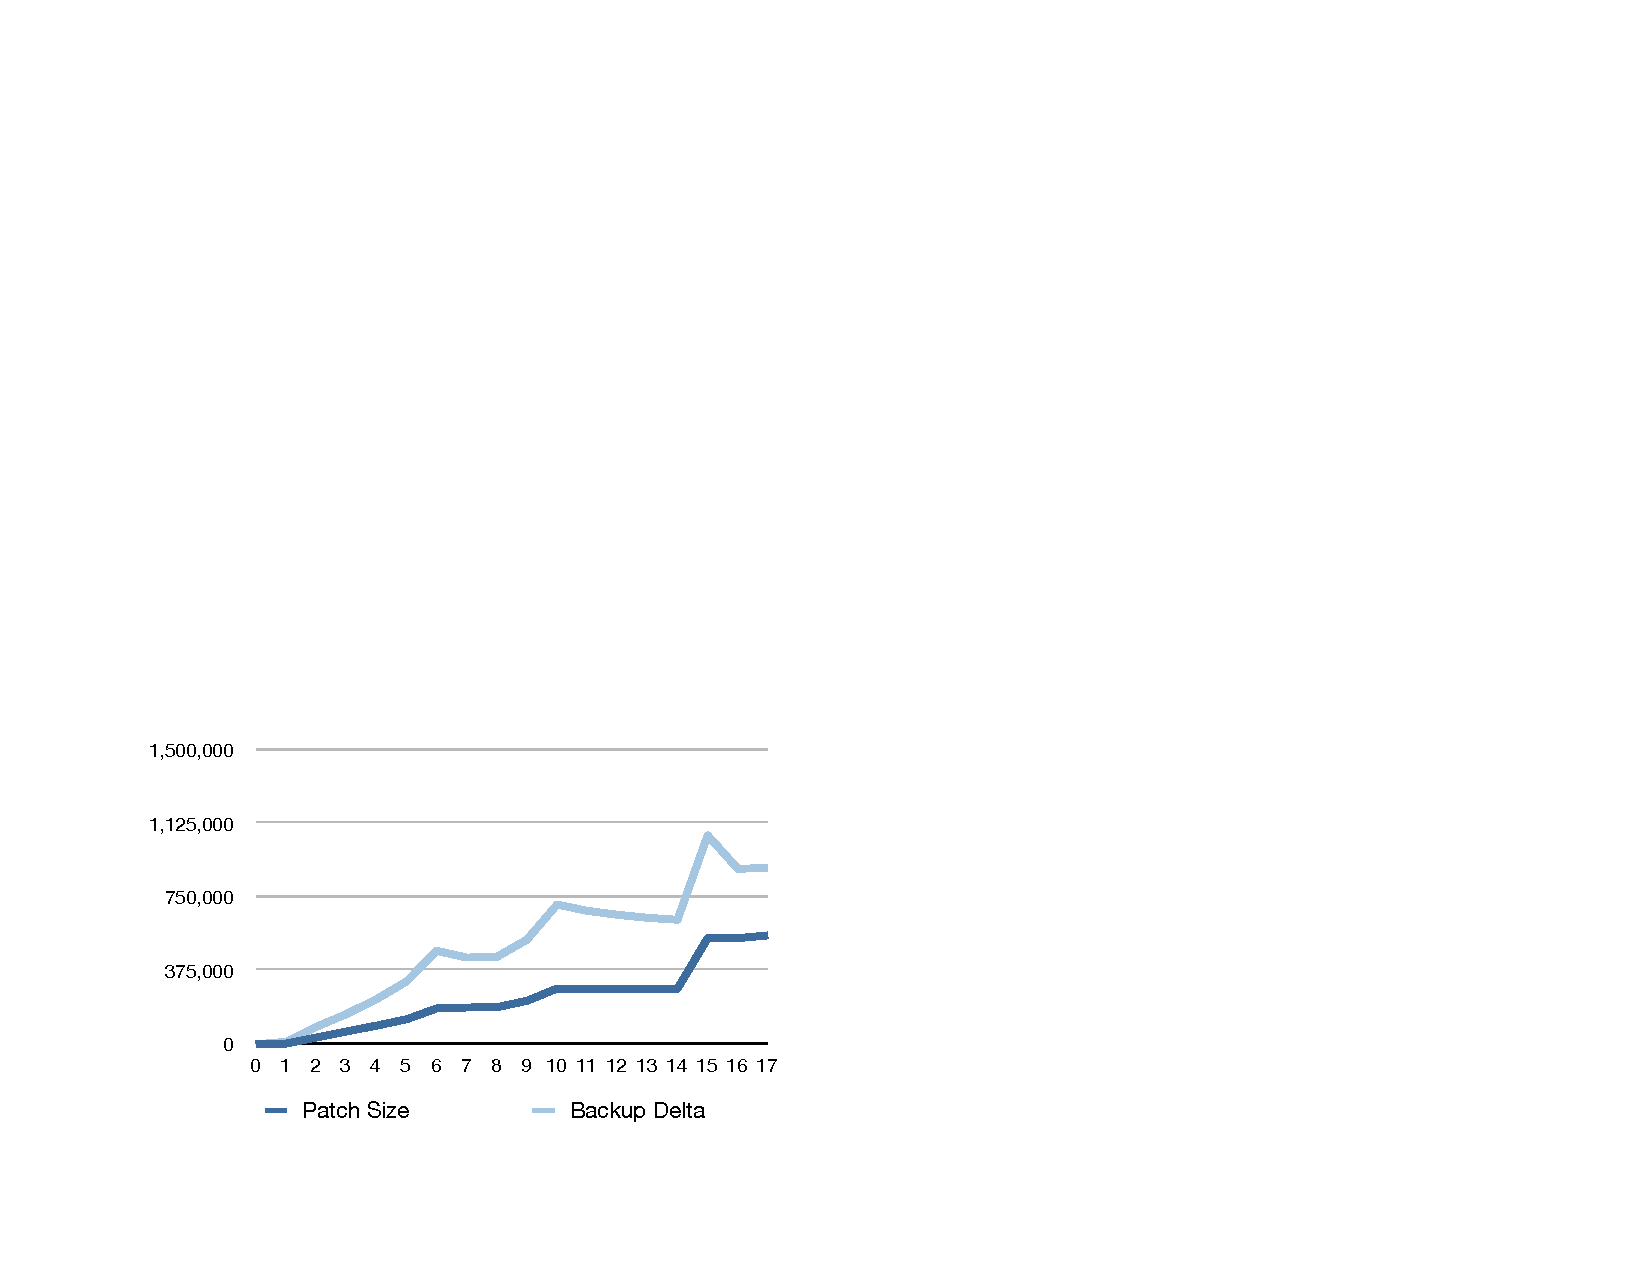
\includegraphics{per-patch-deltas.pdf}}
    \caption{Text patch size and Arrow backup delta}
    \label{graph:per-patch-deltas}
  \end{center}
\end{figure}

\begin{figure}[ht!]
  \begin{center}
    \scalebox{.6}{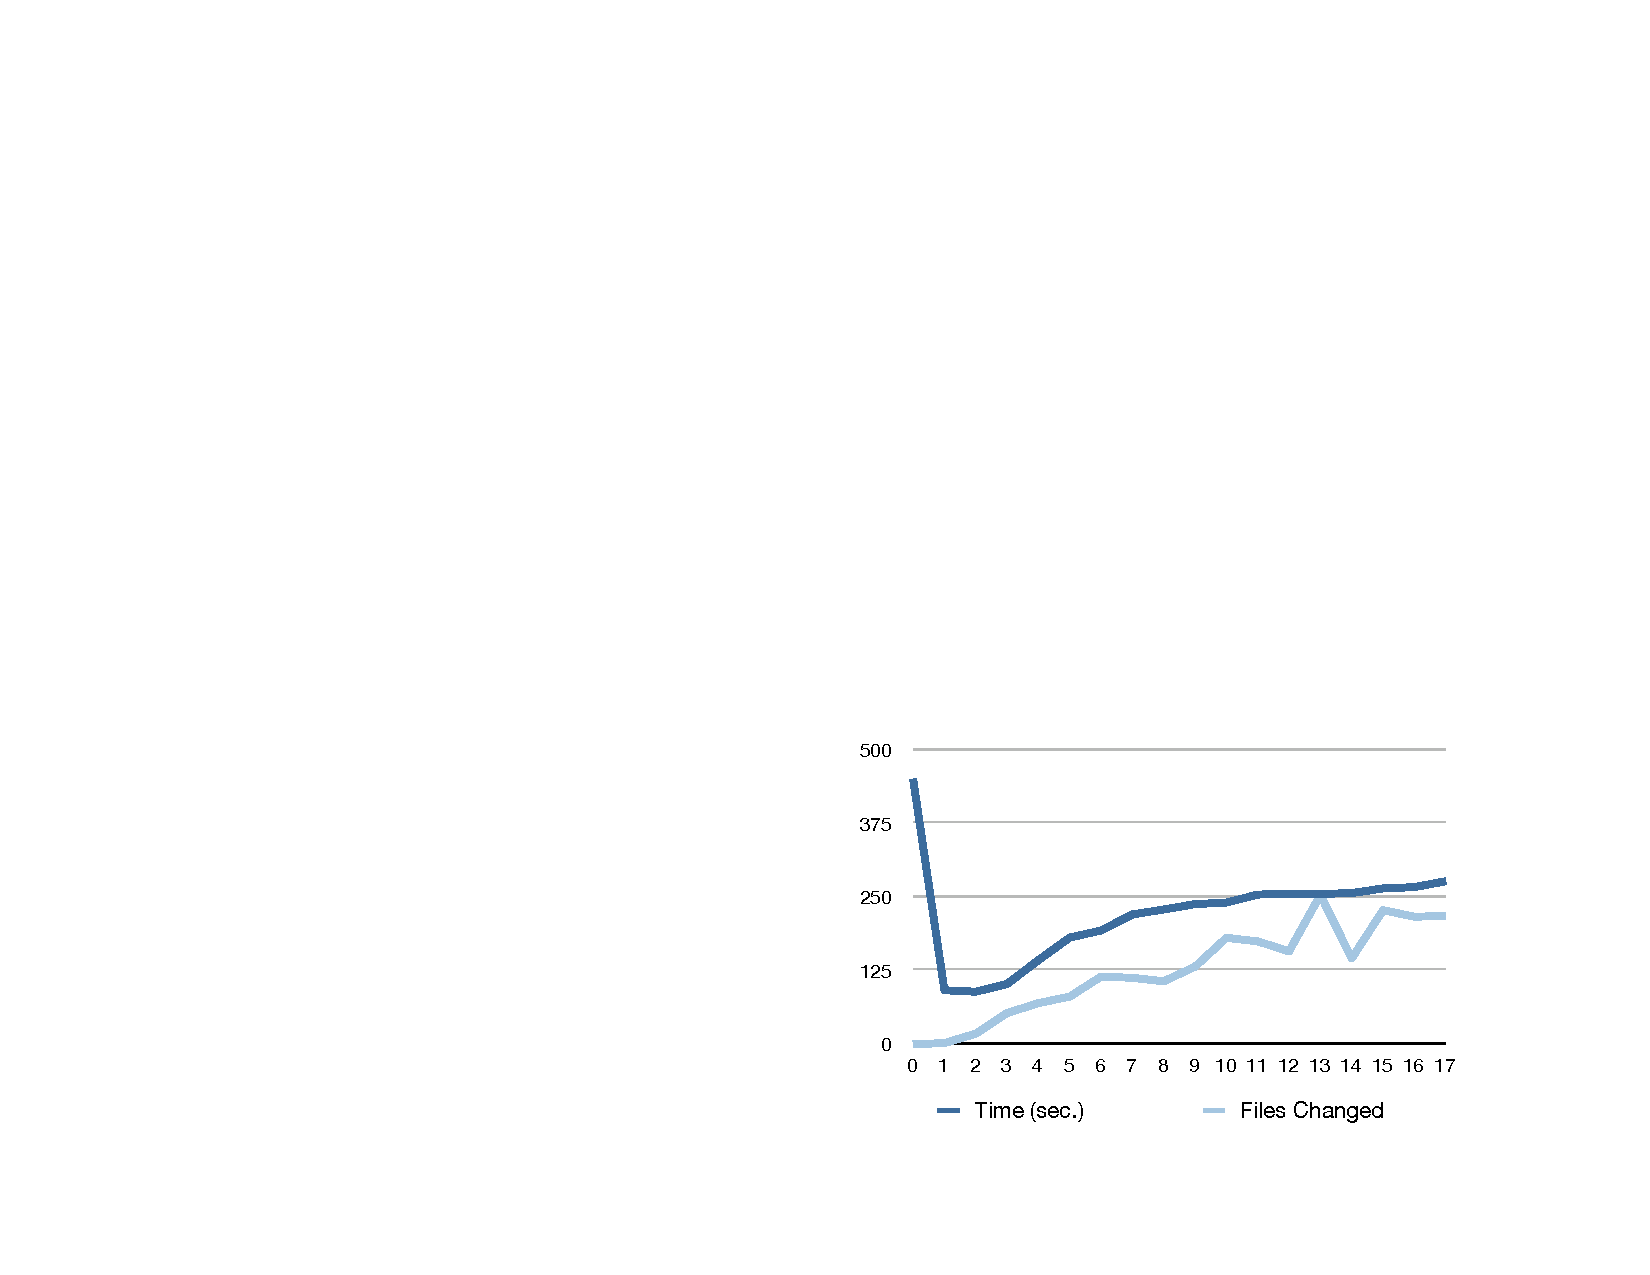
\includegraphics{time-files.pdf}}
    \caption{Backup time and number of files changed}
    \label{graph:time-files}
  \end{center}
\end{figure}

The \emph{patch size} column is the size of the patch file, in bytes,
decompressed. \emph{Source} is the size of the kernel tree with the
patch applied. \emph{Backup} is the size of the Arrow backup, storing
all cumulative version trees, by counting the bytes used by the
symlink tree, the version files, and the chunks used in the block
store (since many slots of the block store may be unused, the actual
disk space used by the backup is significantly larger). \emph{Time} is
the time in seconds it took to synchronize that kernel tree.
\emph{Files} is the number of changed files in that kernel version.

Table~\ref{table:kernel2} lists the sizes of the various parts of
Arrow's storage system, the symlink tree, the version files, and chunk
storage, from the same test against the Linux kernel source. Also
included is the size difference after backing up that patch version.

\begin{table}[ht!]
  \begin{center}
    \begin{tabular}{!{\color[rgb]{.5,.5,.5}\vline}r!{\color[rgb]{.5,.5,.5}\vline}r!{\color[rgb]{.5,.5,.5}\vline}r!{\color[rgb]{.5,.5,.5}\vline}r!{\color[rgb]{.5,.5,.5}\vline}r!{\color[rgb]{.5,.5,.5}\vline}} \hline
      \multicolumn{1}{|>{\columncolor[rgb]{.9,.9,.9}}c|}{\textbf{Patch}} &
      \multicolumn{1}{>{\columncolor[rgb]{.9,.9,.9}}c|}{\textbf{Tree}} &
      \multicolumn{1}{>{\columncolor[rgb]{.9,.9,.9}}c|}{\textbf{Versions}} &
      \multicolumn{1}{>{\columncolor[rgb]{.9,.9,.9}}c|}{\textbf{Chunks}} &
      \multicolumn{1}{>{\columncolor[rgb]{.9,.9,.9}}c|}{\textbf{Difference}} \\ \hline
      \rowcolor{white}
       0 & 6,020,348 & 18,715,460 & 258,371,942 &         0 \\
      \rowcolor[rgb]{.94,.96,.98}
       1 & 6,020,372 & 18,721,280 & 258,378,219 &    12,121 \\
      \rowcolor{white}
       2 & 6,020,372 & 18,763,104 & 258,424,980 &    88,585 \\
      \rowcolor[rgb]{.94,.96,.98}
       3 & 6,020,369 & 18,832,200 & 258,509,619 &   153,732 \\
      \rowcolor{white}
       4 & 6,020,366 & 18,939,252 & 258,632,324 &   229,754 \\
      \rowcolor[rgb]{.94,.96,.98}
       5 & 6,020,371 & 19,108,140 & 258,783,973 &   320,542 \\
      \rowcolor{white}
       6 & 6,020,365 & 19,365,364 & 259,003,428 &   476,673 \\
      \rowcolor[rgb]{.94,.96,.98}
       7 & 6,020,370 & 19,622,648 & 259,188,647 &   442,508 \\
      \rowcolor{white}
       8 & 6,020,368 & 19,883,304 & 259,373,834 &   445,841 \\
      \rowcolor[rgb]{.94,.96,.98}
       9 & 6,020,364 & 20,184,188 & 259,606,858 &   533,904 \\
      \rowcolor{white}
      10 & 6,020,355 & 20,577,220 & 259,926,570 &   712,735 \\
      \rowcolor[rgb]{.94,.96,.98}
      11 & 6,020,366 & 20,971,084 & 260,213,424 &   680,729 \\
      \rowcolor{white}
      12 & 6,020,361 & 21,348,916 & 260,496,343 &   660,746 \\
      \rowcolor[rgb]{.94,.96,.98}
      13 & 6,020,356 & 21,725,972 & 260,764,625 &   645,333 \\
      \rowcolor{white}
      14 & 6,020,361 & 22,099,124 & 261,026,676 &   635,208 \\
      \rowcolor[rgb]{.94,.96,.98}
      15 & 6,020,361 & 22,613,212 & 261,578,665 & 1,066,077 \\
      \rowcolor{white}
      16 & 6,020,366 & 23,116,276 & 261,971,385 &   895,789 \\
      \rowcolor[rgb]{.94,.96,.98}
      \arrayrulecolor[rgb]{.5,.5,.5}
      17 & 6,020,348 & 23,620,716 & 262,365,686 &   898,723 \\ \hline
    \end{tabular}
    \caption{Storage breakdown of Linux kernel versions}
    \label{table:kernel2}
  \end{center}
\end{table}

This next test implemented network backups by tunneling a simple
protocol over an SSH connection. The client side performs the
synchronization, retrieving a version file for a file to be
synchronized, after comparing the file's MD5 hash (the file is not
synchronized if it has clearly not changed); the server side tracks
the chunk store, the version files, and the file tree. The same test
of Linux kernel versions from the previous test, tunneling over the
local loopback device, measuring the time taken and the bytes read and
written. Table~\ref{table:kernel-net} shows the results of this test.

\begin{table}[ht!]
  \begin{center}
    \begin{tabular}{!{\color[rgb]{.5,.5,.5}\vline}r!{\color[rgb]{.5,.5,.5}\vline}r!{\color[rgb]{.5,.5,.5}\vline}r!{\color[rgb]{.5,.5,.5}\vline}r!{\color[rgb]{.5,.5,.5}\vline}} \hline
      \multicolumn{1}{|>{\columncolor[rgb]{.9,.9,.9}}c|}{\textbf{Patch}} &
      \multicolumn{1}{>{\columncolor[rgb]{.9,.9,.9}}c|}{\textbf{Time}} &
      \multicolumn{1}{>{\columncolor[rgb]{.9,.9,.9}}c|}{\textbf{Read}} &
      \multicolumn{1}{>{\columncolor[rgb]{.9,.9,.9}}c|}{\textbf{Written}} \\ \hline
      \rowcolor{white}
       0 & 440.77 &  2,752,454 & 276,687,703 \\
      \rowcolor[rgb]{.94,.96,.98}
       1 &  25.82 &    816,904 &   1,259,019 \\
      \rowcolor{white}
       2 &  17.93 &    851,860 &   1,636,856 \\
      \rowcolor[rgb]{.94,.96,.98}
       3 &  15.48 &    870,087 &   1,487,275 \\
      \rowcolor{white}
       4 &  22.45 &    903,195 &   1,776,221 \\
      \rowcolor[rgb]{.94,.96,.98}
       5 &  79.02 &    975,071 &   2,613,638 \\
      \rowcolor{white}
       6 & 136.64 &  1,062,382 &   2,805,430 \\
      \rowcolor[rgb]{.94,.96,.98}
       7 &  75.39 &  1,066,618 &   1,772,322 \\
      \rowcolor{white}
       8 &  25.66 &  1,075,352 &   1,850,436 \\
      \rowcolor[rgb]{.94,.96,.98}
       9 &  68.07 &  1,113,524 &   2,445,167 \\
      \rowcolor{white}
      10 & 163.88 &  1,202,211 &   3,214,490 \\
      \rowcolor[rgb]{.94,.96,.98}
      11 &  96.83 &  1,202,757 &   2,030,031 \\
      \rowcolor{white}
      12 &  18.58 &  1,202,751 &   2,020,530 \\
      \rowcolor[rgb]{.94,.96,.98}
      13 &  16.68 &  1,205,075 &   2,034,749 \\
      \rowcolor{white}
      14 &  17.91 &  1,208,353 &   2,064,046 \\
      \rowcolor[rgb]{.94,.96,.98}
      15 & 116.60 &  1,333,601 &   4,053,726 \\
      \rowcolor{white}
      16 &  41.00 &  1,335,040 &   2,337,040 \\
      \rowcolor[rgb]{.94,.96,.98}
      \arrayrulecolor[rgb]{.5,.5,.5}
      17 &  28.50 &  1,350,156 &   2,559,890 \\ \hline
    \end{tabular}
    \caption{Network backup of Linux kernel versions}
    \label{table:kernel-net}
  \end{center}
\end{table}

These results are quite in line with what is expected: there is a
constant overhead for transferring the MD5 hashes for all the files in
the backup, and the time needed to compute these hashes. As the
differences increase, it tends to take longer and more bytes
transferred, including the MD5 hashes, the contents of each version
file for those files where the MD5 checksum did not match, and the new
file chunks. The overhead for the initial backup is about 12\% greater
than the data, and about 10\% more needs to be sent over the
network. Compared with backing up the an entire kernel version, Arrow
only needed to transfer at most 2\% of the total size of the source
data (for the biggest incremental delta, version 2.6.23.15), and
storing this new version only increased the backup size by 0.4\% of
the new version size; or, about 11\% of the size of the \texttt{bzip2}
compressed tar archive sent over the wire, and about 2\% increase in
storage.

All these tests were run on a low-end Ubuntu Linux server, with a
two-core 2.8GHz Intel Pentium D and 1GB of RAM, backing up to a single
7200 RPM hard disk.

This final test increased the size of blocks from around 200 entries
to 5,000, as an effort to reduce I/O load. The test used the local C
client to back up every major point release kernel from version 2.6.10
to 2.6.25, representing almost three and a half years of
development. This test was run on the same machine as before, and also
on a server-class system with two four-core 3.2 GHz Intel Xeon
processors, 8 GB of RAM, and backing up to a five-disk RAID 5
array. The difference in performance is startling, illustrated in
table~\ref{table:big-kernel} and figure~\ref{graph:big-kernel}. The
reason for this seems to be that arrow is heavily I/O bound; running a
similar test under a \texttt{dtrace} session on Mac OS X revealed that
most of the program time is spent in \texttt{fread}, \texttt{open} and
\texttt{close}, \texttt{memcpy} (the blocks are implemented by mapping
the block file into memory), and \texttt{munmap}. These results do
seem to suggest that Arrow requires a certain amount of disk bandwidth
to operate quickly, and that it can saturate a low-bandwidth disk
after a modest amount of data is written to it. This raises an
important issue with a linear hash table: writes that should be
essentially sequential are randomized across the disk; we can't help
the case where we are referencing an existing chunk, but adjascent
chunks in a single file are scattered throughout the storage system,
and in certain cases, doing this scattering can be very expensive.

\begin{table}
  \begin{center}
    \begin{tabular}{!{\color[rgb]{.5,.5,.5}\vline}r!{\color[rgb]{.5,.5,.5}\vline}r!{\color[rgb]{.5,.5,.5}\vline}r!{\color[rgb]{.5,.5,.5}\vline}r!{\color[rgb]{.5,.5,.5}\vline}r!{\color[rgb]{.5,.5,.5}\vline}r!{\color[rgb]{.5,.5,.5}\vline}} \hline
      \multicolumn{1}{|>{\columncolor[rgb]{.9,.9,.9}}c|}{\textbf{Kernel}} &
      \multicolumn{1}{>{\columncolor[rgb]{.9,.9,.9}}c|}{\textbf{Files}} &
      \multicolumn{1}{>{\columncolor[rgb]{.9,.9,.9}}c|}{\textbf{Time (1 disk)}} &
      \multicolumn{1}{>{\columncolor[rgb]{.9,.9,.9}}c|}{\textbf{Time (RAID-5)}} &
      \multicolumn{1}{>{\columncolor[rgb]{.9,.9,.9}}c|}{\textbf{Size}} &
      \multicolumn{1}{>{\columncolor[rgb]{.9,.9,.9}}c|}{\textbf{Delta}} \\ \hline
      \rowcolor{white}
      2.6.10 & 16,583 &  263.82 & 150.50 &   219,538,292 &           0 \\
      \rowcolor[rgb]{.94,.96,.98}
      2.6.11 &  5,481 &   50.42 &  24.16 &   249,878,382 &  30,340,090 \\
      \rowcolor{white}
      2.6.12 &  7,313 &   89.42 & 111.70 &   294,696,204 &  44,817,822 \\
      \rowcolor[rgb]{.94,.96,.98}
      2.6.13 &  8,285 &  162.65 & 154.36 &   348,544,181 &  53,847,977 \\
      \rowcolor{white}
      2.6.14 &  8,517 &  428.72 & 130.97 &   399,782,781 &  51,238,600 \\
      \rowcolor[rgb]{.94,.96,.98}
      2.6.15 &  9,258 &  436.17 & 101.68 &   460,175,258 &  60,392,477 \\
      \rowcolor{white}
      2.6.16 & 10,051 &  236.86 & 124.06 &   526,137,368 &  65,962,110 \\
      \rowcolor[rgb]{.94,.96,.98}
      2.6.17 & 10,247 &  194.90 & 257.49 &   594,133,084 &  67,995,716 \\
      \rowcolor{white}
      2.6.18 & 11,768 &  278.77 & 106.34 &   666,703,249 &  72,570,165 \\
      \rowcolor[rgb]{.94,.96,.98}
      2.6.19 & 12,471 &  967.12 & 135.16 &   748,048,042 &  81,344,793 \\
      \rowcolor{white}
      2.6.20 & 11,801 &  807.57 &  97.71 &   819,728,218 &  71,680,176 \\
      \rowcolor[rgb]{.94,.96,.98}
      2.6.21 & 11,782 &  853.37 &  96.82 &   896,486,021 &  76,757,803 \\
      \rowcolor{white}
      2.6.22 & 12,576 &  944.28 & 105.83 &   982,696,828 &  86,210,807 \\
      \rowcolor[rgb]{.94,.96,.98}
      2.6.23 & 12,231 &  973.92 & 167.14 & 1,065,769,264 &  83,072,436 \\
      \rowcolor{white}
      2.6.24 & 13,413 &  995.01 & 182.68 & 1,162,798,886 &  97,029,622 \\
      \rowcolor[rgb]{.94,.96,.98}
      \arrayrulecolor[rgb]{.5,.5,.5}
      2.6.25 & 13,940 & 1185.11 & 111.60 & 1,266,597,571 & 103,798,685 \\ \hline
    \end{tabular}
    \caption{Native, local backup of major kernel releases}
    \label{table:big-kernel}
  \end{center}
\end{table}

\begin{figure}[ht!]
  \begin{center}
    \scalebox{.6}{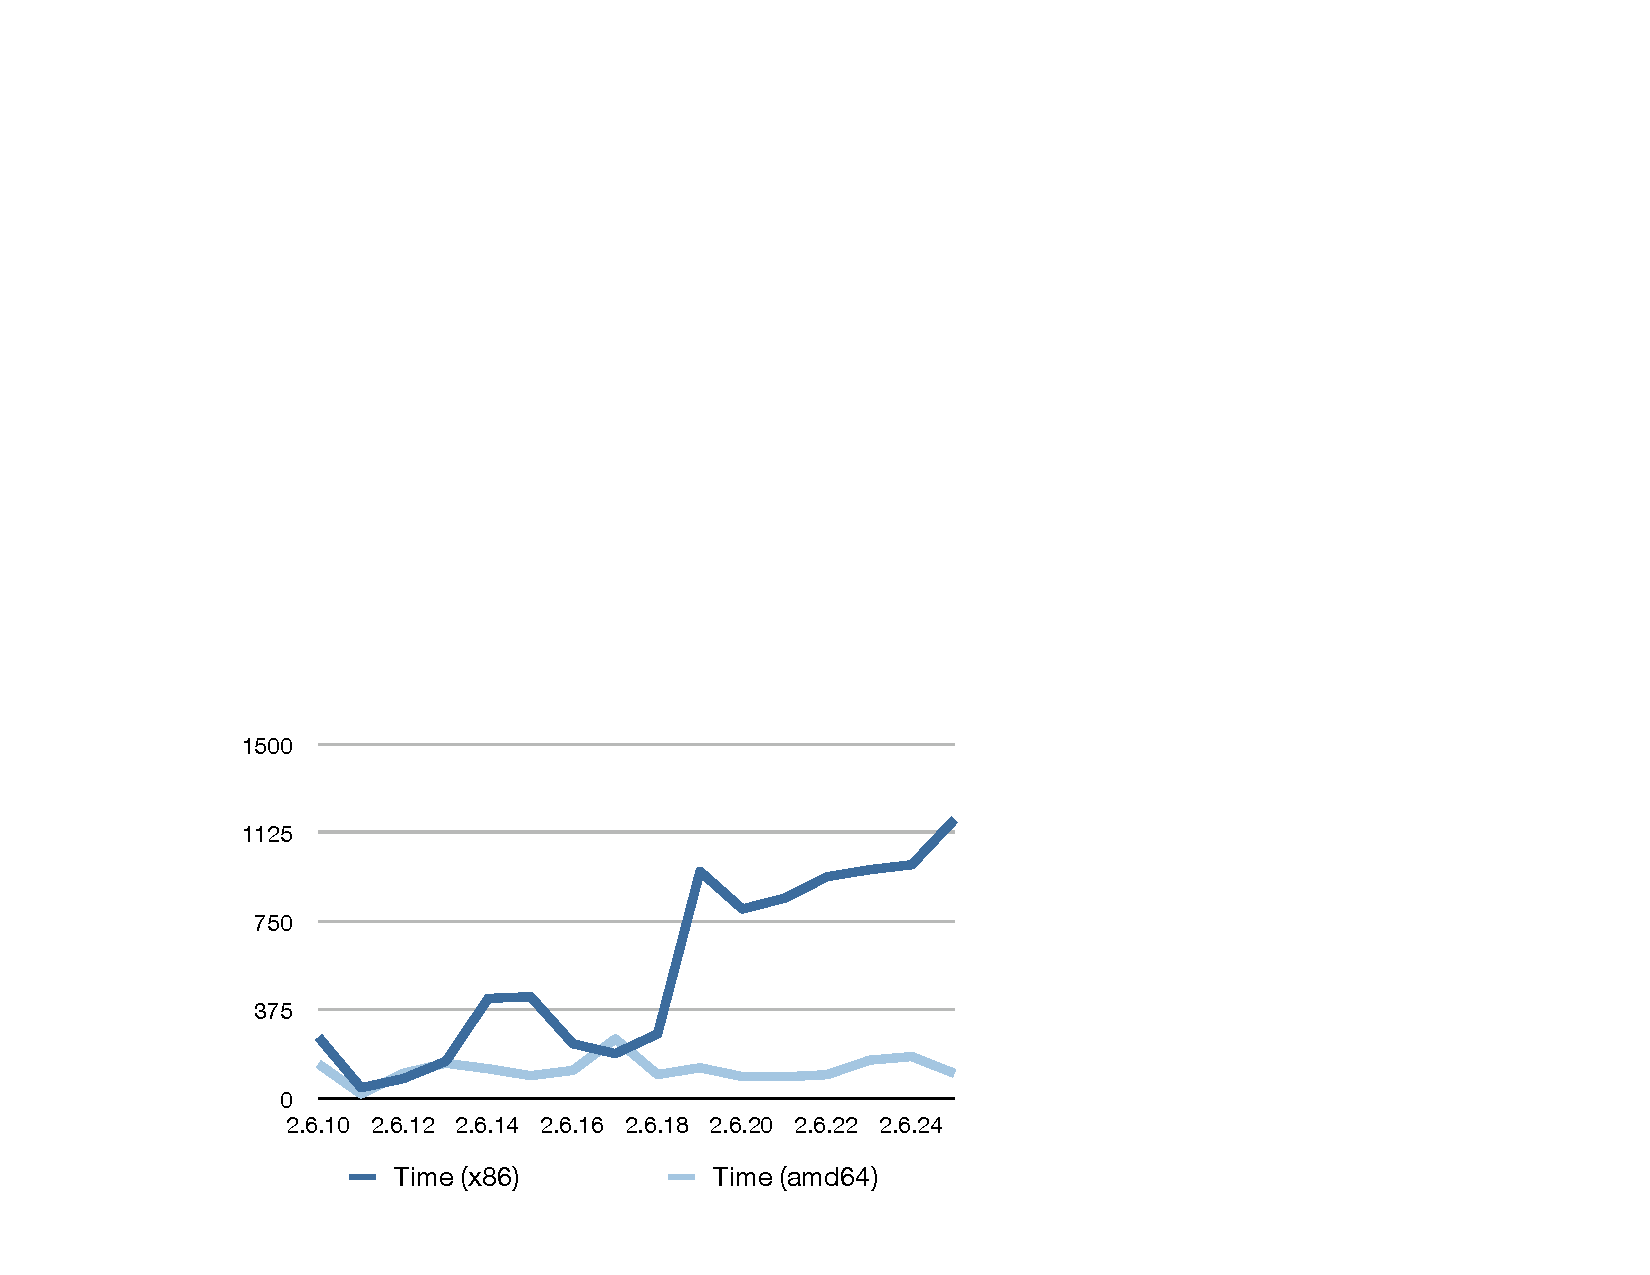
\includegraphics{thats-not-a-knife.pdf}}
    \caption{Arrow on commodity (x86) and server (amd64) hardware}
    \label{graph:big-kernel}
  \end{center}
\end{figure}

\pagebreak

\section{Conclusions}

Arrow is a new application of existing ideas, combining them into a
safe, efficient, recoverable data backup system. The current
implementation is only a prototype, but proves that the idea can offer
a data backup solution that combines storage and transmission
efficiency, and strong error detection and correction.

Arrow is still only a beginning. There are many other concerns with
archival storage and data backup that are not addressed here. Most
especially is distributing the storage across multiple storage
systems; for a truly reliable backup system, it can't rely on a single
piece of hardware, or a single software system. Arrow's implementation
of various pieces introduces some performance bottlenecks, most
clearly when the backup size grows very large, which could be
addressed separately. To be fully usable as an archival storage
system, Arrow still needs support and optimization of the verification
and correction processes, and needs a usable method for restoring
backed-up data.

%% Uncomment this for publishing on the intarwebs
%\section{Licensing}

% Arrow makes use of a Reed-Solomon library, copyright \copyright\
% 2007 by Kevin Greenan, and others from UCSC; the \texttt{bstrlib}
% string library, copyright \copyright\ 2002--2007 Paul Hsieh; parts
% of librsync, copyright \copyright\ 2000, 2001 Martin Pool and
% \copyright\ 2003 Donovan Baarda; and a simple base-64 encoder,
% copyright \copyright\ 1996, 2002 by Richard Faith.

% Arrow is copyright \copyright\ 2008 Casey Marshall.

% Arrow is free software: you can redistribute it and/or modify it under
% the terms of the GNU General Public License as published by the Free
% Software Foundation, either version 3 of the license, or (at your
% option) any later version.

% Arrow is distributed in the hope that it will be useful, but
% \emph{without any warranty;} without even the implied warranty of
% \emph{merchantability} or \emph{fitness for a particular purpose.}
% See the GNU General Public License for more details.

% You should have received a copy of the GNU General Public License
% along with Arrow. If not, see \url{http://www.gnu.org/licenses/}.

% This report is licensed under the Creative Commons Attribution-No
% Derivative Works 3.0 United States License. For the full terms, see
% \url{http://creativecommons.org/licenses/by-nd/3.0/us/}.

% Arrow is available via a git repository at
% \url{http://git.metastatic.org/}. A read-only repository is
% available at \url{http://git.metastatic.org/readonly/arrow.git}. It
% is written in C, and runs on GNU/Linux and Mac OS X.

\bibliography{sources}
\end{document}
